\documentclass{article}
\usepackage{tikz}
\usetikzlibrary{graphs, positioning}

\begin{document}

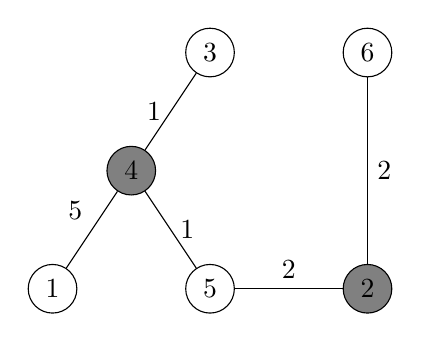
\begin{tikzpicture}
    % Define nodes
    \node[shape=circle,draw=black] (1) at (0,0) {1};
    \node[shape=circle,draw=black,fill=gray] (2) at (4,0) {2};
    \node[shape=circle,draw=black] (3) at (2,3) {3};
    \node[shape=circle,draw=black,fill=gray] (4) at (1,1.5) {4};
    \node[shape=circle,draw=black] (5) at (2,0) {5};
    \node[shape=circle,draw=black] (6) at (4,3) {6};
    % Draw edges
    \draw (1) -- node[above left] {5} (4);
    \draw (4) -- node[left] {1} (3);
    \draw (4) -- node[right] {1} (5);
    \draw (5) -- node[above] {2} (2);
    \draw (2) -- node[right] {2} (6);

\end{tikzpicture}

\end{document}